\chapter{Related Work}
\label{chapter:related}

While looking for works related to this one, we searched for works that focused on dungeon or content generation specifically for games and also for works that had their focus on cave generation.

\section{Conditional Convolutional Generative
Adversarial Networks Based Interactive
Procedural Game Map Generation}

This paper by \citeauthor{ping:2020} suggests the usage of Conditional Generative Adversarial Network and Convolutional Neural Network to create a game design system. The system takes by input a gameplay area map defined by the user and generates a complex map with the same design pattern.

\begin{figure}[h]
    \caption{Example of the system's usage}
    \centerline{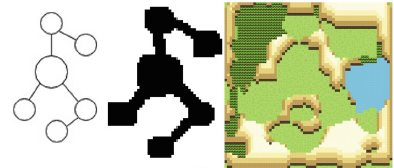
\includegraphics{images/related_work/ping.png}}
    \legend{Source: \cite{ping:2020}}
    \label{fig:ping}
\end{figure}
In Figure \ref{fig:ping} we see in the first two steps the image designed by the user and in the last step the generated map. The variety of the maps depend on the training of the network as well \citeyear{ping:2020}.

\section{Cellular automata for real-time generation
of infinite cave levels}

In this paper a simple cellular automata (CA) algorithm is used in order to generate, in real time, infinite cave-like levels. The algorithm was tested in a game called Cave Crawler, which is a birds-eye view game where the players have to traverse the generated tunnels while defeating waves of enemies. 

Much like this paper, our work also utilizes a simple CA algorithm as one of the steps of the system in order to generate the cave levels, but on this paper the focus is more on the real-time and performance aspect of the map generation \cite{johnson:2010}.

\section{Procedural creation of 3D solution cave models}

The focus of this article by \citeauthor{boggus:2009} is to use PCG algorithms to create 3D cave models based on real cave patterns. They present the usage of surface images of cave patterns and apply these images to create models of cave systems. The surface images can be generated, for example by utilizing fractal algorithms, or real world terrain data.

After the surface image is provided, they create a heightmap out of it and then simulate the flow of water through this map, since this is ultimately the way solution caves are formed. Figure \ref{fig:3d_cave} shows a cross section view of a generated cave, where lighter areas represent walls \citeyear{boggus:2009}.
\begin{figure}[h]
    \caption{Spongework cave pattern}
    \centerline{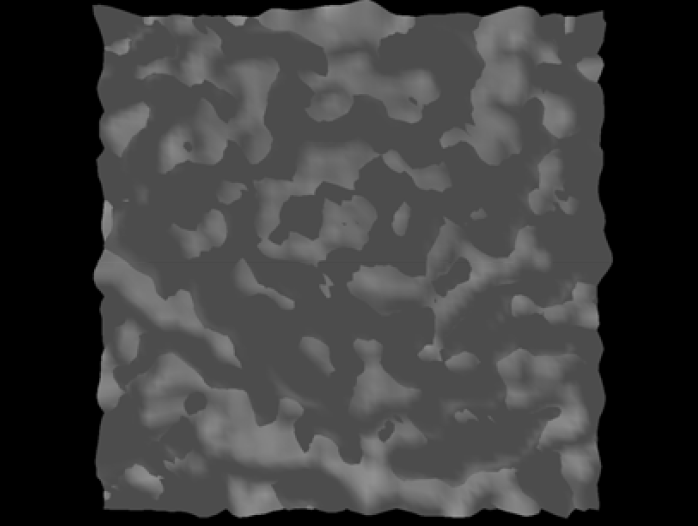
\includegraphics[width=7cm]{images/related_work/3d_cave.png}}
    \legend{Source: \cite{boggus:2009}}
    \label{fig:3d_cave}
\end{figure}

\section{Procedural Playable Cave Systems
based on Voronoi Diagram and Delaunay Triangulation}

This paper by \citeauthor{santamaria:2014} presents a new method for 2D or 3D playable cave systems to be generated. The user-defined input for their method are a list of points of interest (POI) that will be put inside the cave and the relationship between these POI. The paper defines a list of parameters that compose the POI like location, depth, number of branches etc.

\begin{figure}[h]
    \caption{Cave generation process}
    \centerline{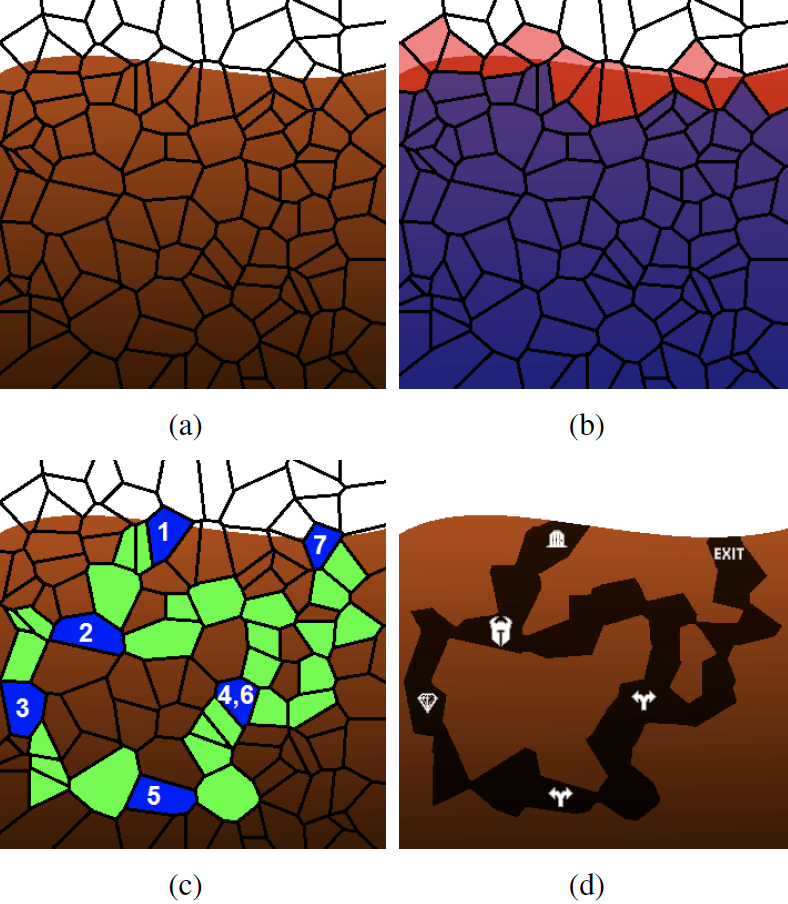
\includegraphics[width=6cm]{images/related_work/poi_cave.png}}
    \legend{Source: \cite{santamaria:2014}}
    \label{fig:poi_cave}
\end{figure}

Figure \ref{fig:poi_cave} shows their cave generation process. In (a) a Voronoi diagram is generated on a terrain representation. (b) shows the classification of the cells. (c) shows 7 POI assigned to their respective cells in the diagram and (d) shows the final generated cave \citeyear{santamaria:2014}.

\section{Analysis and Development of a
Game of the Roguelike Genre}

This work describe the development of a prototype game of the roguelike genre, and presents an analysis focused on the different techniques used on the AI for enemies and on the procedural generation of the dungeons. The compared PCG algorithms include: Kruskal and Prim, both being genetic algorithms; depth-first search, used to generate perfect mazes and cellular automata for cave-like structures. Some of the gathered results show that techniques of basic interaction iteration and BSP trees have good scalability while cellular automata and depth-first search need optimization or restriction in other to increase scalability \cite{goncalves:2015}.
